\documentclass{article}

\usepackage[utf8]{inputenc}
\usepackage[russian, french]{babel}
\usepackage{amsthm}
\usepackage{amsmath}
\usepackage{mathtools}
\usepackage{amssymb}
\usepackage[symbol]{footmisc}
\usepackage{graphicx}
\usepackage{tikz}

\graphicspath{ {./images/} }

\title{Сходимость}
\author{Роман Кушниренко}

\makeatletter
\newcommand*{\rom}[1]{\expandafter\@slowromancap\romannumeral #1@}
\makeatother

\renewcommand{\thefootnote}{\fnsymbol{footnote}}
\renewcommand*{\dotFFN}{}

\newtheorem{theorem}{Теорема}[section]
\newtheorem*{lemma}{Лемма}
\newtheorem{claim}{Утверждение}[section]
\newtheorem{example}{Пример}
\newtheorem{definition}{Определение}[section]
\newtheorem*{consequence}{Следствие}

\DeclareMathOperator*\lowlim{\underline{lim}}
\DeclareMathOperator*\uplim{\overline{lim}}

\begin{document}

	\selectlanguage{russian}

	\maketitle

	\section{Последовательность и ее предел}

\begin{definition}
Последовательность \(\{x_n\}\) в метрическом пространстве \(X\) называется сходящейся, если существует точка \(x \in X\), обладающая следующим свойством: для каждого \(\varepsilon > 0\) существует целое число \(N\), такое, что при \(n \geq N\) имеем \(\rho(x_n, x) < \varepsilon\) (здесь \(\rho\) обозначает расстояние в \(X\)).

В этом случае мы будем говорить также, что последовательность \(\{x_n\}\) сходится к \(x\) или что \(x\) \(-\) предел последовательности \(\{x_n\}\), и будем писать \(x_n \to x\) или
\[
\lim_{n \to \infty} x_n = x.
\]
\end{definition}

Следующая теорема показывает корректность этого определения.

\begin{theorem}
Если \(x \in X\), \(x' \in X\) и \(\{x_n\}\) сходится к \(x\) и к \(x'\), то \(x = x'\).
\end{theorem}

\begin{proof}
Пусть задано число \(\varepsilon > 0\). Тогда существуют целые числа \(N\), \(N'\), такие, что \(n \geq N\) влечет за собой \(2\rho(x_n, x) < \varepsilon\), а \(n \geq N'\) влечет за собой \(2\rho(x_n, x') < \varepsilon\).

Значит, если \(n \geq \max(N, N')\), то
\[
\rho(x, x') \leq \rho(x, x_n) + \rho(x_n, x') < \varepsilon.
\]

Вследствие произвольности числа \(\varepsilon\) заключаем, что \(\rho(x, x') = 0\).
\end{proof}

\begin{definition}
Если последовательность \(\{x_n\}\) не сходится, то говорят, что она расходится.
\end{definition}

Сформулируем теперь некоторые важные свойства сходящихся последовательностей в метрических пространствах.

\begin{theorem}
Последовательность \(\{x_n\}\) в метрическом пространстве \(X\) сходится к \(x \in X\) тогда и только тогда, когда каждая окрестность точки \(x\) содержит все члены последовательности \(\{x_n\}\), за исключением конечного их числа.
\end{theorem}

\begin{proof}
Допустим, что \(x_n \to x\), и пусть \(O_\varepsilon(x)\) \(-\) окрестность точки \(x\) для некоторого \(\varepsilon > 0\). Этому \(\varepsilon\) соответствует \(N\), такое, что из неравенства \(n \geq N\) следует, что \(\rho(x_n, x) < \varepsilon\). Таким образом, неравенство \(n \geq N\) влечет за собой включение \(x_n \in O_\varepsilon(x)\).

Обратно, допустим, что каждая окрестность точки \(x\) содержит все точки \(x_n\), кроме конечного их числа. Зафиксируем \(\varepsilon > 0\), и пусть \(O_\varepsilon(x)\) \(-\) окрестность точки \(x\). По предположению, существует \(N\), такое, что \(x_n \in O_\varepsilon(x)\), если \(n \geq N\). Таким образом, \(\rho(x_n, x) < \varepsilon\), если \(n \geq N\); значит, \(x_n \to x\).
\end{proof}

\begin{theorem}
Пусть \(\{x_n\}\) \(-\) последовательность в метрическом пространстве \(X\). Если \(\{x_n\}\) сходится, то \(\{x_n\}\) ограничена.
\end{theorem}

\begin{proof}
Допустим, что \(x_n \to x\). Тогда существует целое \(N\), такое, что при \(n > N\) имеем \(\rho(x, x_n) < 1\). Положим
\[
r = \max\{1, \rho(x, x_1), ..., \rho(x, x_N)\}.
\]
Тогда \(x_n \in B[x, r]\) при \(n \in \mathbb{N}\).
\end{proof}

\begin{theorem}
Если \(x\) \(-\) предельная точка множества \(M \subset X\), то существует последовательность \(\{x_n\}\) элементов множества \(M\), такая, что \(x = \lim\limits_{n \to \infty} x_n\).
\end{theorem}

\begin{proof}
Для каждого положительного целого \(n\) существует точка \(x_n \in M\), такая, что \(\rho(x_n, x) < {{1} \over {n}}\). Для данного \(\varepsilon > 0\) выберем \(N\) так, что \(N > {1 \over \varepsilon}\). Если \(n > N\), то \(\rho(x_n, x) < {1 \over n} < {1 \over N} < \varepsilon\). Значит, \(x_n \to x\).
\end{proof}

\section{Сходимость и арифметические операции}

Для последовательностей вещественных чисел мы можем изучать соотношения между сходимостью, с одной стороны, и арифметическими операциями, с другой.

\begin{theorem}
Допустим, что \(\{s_n\}\), \(\{t_n\}\) \(-\) последовательности вещественных чисел и \(\lim\limits_{n \to \infty} s_n = s\), \(\lim\limits_{n \to \infty} t_n = t\). Тогда
\begin{enumerate}
    \item \(\lim\limits_{n \to \infty} (s_n + t_n) = s + t\);
    \item \(\lim\limits_{n \to \infty} cs_n = cs\), \(\lim\limits_{n \to \infty} (c + s_n) = c + s\) для любого числа \(c\);
    \item \(\lim\limits_{n \to \infty} {s_n}{t_n} = st\);
    \item \(\lim\limits_{n \to \infty} {1 \over s_n} = {1 \over s}\), если только \(s_n \neq 0\) \(\forall n \in \mathbb{N}\) и \(s \neq 0\).
\end{enumerate}
\end{theorem}
\pagebreak
\begin{proof}
  \(\newline\)
\begin{enumerate}
    \item Для данного \(\varepsilon > 0\) существуют \(N\), \(N' \in \mathbb{N}\), такие, что при \(n \geq N\) имеем \(2|s_n - s| < \varepsilon\), а при \(n \geq N'\) имеем \(2|t_n - t| < \varepsilon\). Значит, если \(n \geq \max(N, N')\), то
    \[
    |(s_n + t_n) - (s + t)| \leq |s_n - s| + |t_n - t| < \varepsilon.
    \]
    Вследствие произвольности числа \(\varepsilon\) заключаем, что \(\lim\limits_{n \to \infty} (s_n + t_n) = s + t\).
    \item Тривиально.
    \item Для данного \(\varepsilon > 0\) существуют \(N\), \(N' \in \mathbb{N}\), такие, что при \(n \geq N\) имеем \(|s_n - s| < \sqrt{\varepsilon}\), а при \(n \geq N'\) имеем \(|t_n - t| < \sqrt{\varepsilon}\). Значит, если \(n \geq \max(N, N')\), то
    \[
    |(s_n - s)(t_n - t)| < \varepsilon.
    \]
    Тогда вследствие произвольности числа \(\varepsilon\)
    \[
    \lim\limits_{n \to \infty} (s_n - s)(t_n - t) = 0.
    \]
    Воспользуемся теперь тождеством
     \[
    s_nt_n - st = (s_n - s)(t_n - t) + s(t_n - t) + t(s_n - s).
    \]
    Переходя к пределу в каждом слагаемом (вследствие \textit{1}) и вынося постоянные за знак предела (вследствие \textit{2}), получим, что
    \[
    \lim\limits_{n \to \infty} (s_nt_n - st) = \lim\limits_{n \to \infty} (s_n - s)(t_n - t) + s\lim\limits_{n \to \infty} t_n - st + t\lim\limits_{n \to \infty} s_n - ts = 0.
    \]
    С другой стороны,
    \[
    \lim\limits_{n \to \infty} (s_nt_n - st)  = \lim\limits_{n \to \infty} {s_nt_n} - st,
    \]
    откуда \(\lim\limits_{n \to \infty} {s_n}{t_n} = st\).
    \item Выбрав \(N\) так, что \(2|s_n - s| < |s|\) при \(n \geq N\), мы видим, что
    \[
    |s| - |s_n| \leq ||s| - |s_n|| \leq |s_n - s| < {|s| \over 2},
    \]
    откуда \(\forall n \geq N\)
    \[
    |s_n| > {|s| \over 2}.
    \]
    Для данного \(\varepsilon > 0\) существует \(N' \in \mathbb{N}\) , такое, что при \(n \geq N'\) имеем
    \[
    |s_n - s| < {|s|^2 \over 2}\varepsilon.
    \]
    Значит, если \(n \geq \max(N, N')\), то
    \[
    \left|{1 \over s_n} - {1 \over s}\right| = \left|{{s_n - s} \over s_ns}\right| < {1 \over |s|} \cdot {|s|^2 \over 2}\varepsilon \cdot {2 \over |s|} = \varepsilon \Leftrightarrow \lim\limits_{n \to \infty} {1 \over s_n} = {1 \over s}.
    \]
\end{enumerate}
\end{proof}

\section{Предельный переход и неравенства}

\begin{theorem}
Пусть \(\{s_n\}\), \(\{t_n\}\) \(-\) две сходящиеся последовательности вещественных чисел, причем \(\lim\limits_{n \to \infty} s_n = s\), \(\lim\limits_{n \to \infty} t_n = t\). Если \(s < t\), то найдется номер \(N \in \mathbb{N}\) такой, что при любом \(n \geq N\) выполнено неравенство \(s_n < t_n\).
\end{theorem}

\begin{proof}
Возьмем число \(u\) такое, что \(s < u < t\). По определению предела найдем числа \(N'\) и \(N''\) так, чтобы при любом \(n \geq N'\) иметь \(|s_n - s| < u - s\) и при любом \(n \geq N''\) иметь \(|t_n - t| < t - u\). Тогда при \(n \geq N = \max(N', N'')\) получим \(s_n < s + (u - s) = u = t - (t - u) < t_n\).
\end{proof}

\begin{consequence}
Пусть \(\lim\limits_{n \to \infty} s_n = s\) и \(\lim\limits_{n \to \infty} t_n = t\). Если существует номер \(N\) такой, что при любом \(n \geq N\) выполнено неравенство \(s_n > t_n\) (\(s_n \geq t_n\)), то \(s \geq t\).
\end{consequence}

\begin{proof}
От противного.
\end{proof}

Стоит заметить, что строгое неравенство в пределе может перейти в равенство. Например, \({1 \over n} > 0\) при любом \(n \in \mathbb{N}\), но \(\lim\limits_{n \to \infty} {1 \over n} = 0\).

\begin{theorem}[Théorème des gendarmes]
Пусть последовательности \(\{s_n\}\), \(\{u_n\}\), \(\{t_n\}\) таковы, что при любом \(n \geq N \in \mathbb{N}\) имеет место соотношение \(s_n \leq u_n \leq t_n\). Если при этом последовательности \(\{s_n\}\), \(\{t_n\}\) сходятся к одному и тому же пределу, то последовательность \(\{u_n\}\) также сходится, причем к этому же пределу.
\end{theorem}

\begin{figure}[h]
\centering
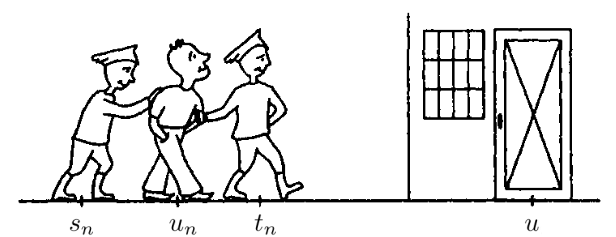
\includegraphics[scale=0.35]{SqueezeTheorem}
\end{figure}

\begin{proof}
Пусть \(\lim\limits_{n \to \infty} s_n = \lim\limits_{n \to \infty} t_n = u\). По \(\varepsilon > 0\) найдем числа \(N' \geq N\) и \(N'' \geq N\) так, чтобы при любом \(n \geq N'\) иметь \(u - \varepsilon < s_n\) и при любом \(n \geq N''\) иметь \(t_n < u + \varepsilon\). Тогда при \(n \geq \max(N', N'')\) получим \(u - \varepsilon < s_n \leq u_n \leq t_n < u + \varepsilon\) или \(|u_n - u| < \varepsilon \Leftrightarrow u = \lim\limits_{n \to \infty} u_n\).
\end{proof}

\section{Некоторые специальные последовательности}

Теперь мы вычислим пределы некоторых часто встречающихся последовательностей.

\begin{theorem}
\(\newline\)
\begin{enumerate}
  \item Если \(p > 0\), то
  \[
  \lim\limits_{n \to \infty} {1 \over {n ^ p}} = 0.
  \]
  \item Если \(p > 0\), то \(\lim\limits_{n \to \infty} {\sqrt[\leftroot{3}\uproot{3}n]{p}} = 1\).
  \item \(\lim\limits_{n \to \infty} {\sqrt[\leftroot{3}\uproot{3}n]{n}} = 1\).
  \item Если \(p > 0\) и \(\alpha \in \mathbb{R}\), то
  \[
  \lim\limits_{n \to \infty} {{n ^ \alpha} \over {(1 + p) ^ n}} = 0.
  \]
  \item Если \(|x| < 1\), то \(\lim\limits_{n \to \infty} {x ^ n} = 0\).
  \item Если \(\alpha \in \mathbb{R}\), то
  \[
  \lim\limits_{n \to \infty} {{\alpha ^ n} \over {n!}} = 0.
  \]
\end{enumerate}
\end{theorem}

\begin{proof}
\(\newline\)
\begin{enumerate}
  \item Возьмем \(N > \left({1 \over \varepsilon}\right)^{1 \over p}\).
  \item Если \(p > 1\), то положим \(x_n = {\sqrt[\leftroot{3}\uproot{3}n]{p}} - 1\). Тогда \(x_n > 0\) и, согласно теореме о биноме,
  \[
  1 + nx_n \leq (1 + x_n)^n = p,
  \]
  так что
  \[
  0 < x_n \leq {{p - 1} \over n}.
  \]
  Значит, \(x_n \to 0\) (в силу теоремы 3.2). Если \(p = 1\), то утверждение очевидно; если \(0 < p < 1\), то результат получается переходом к обратным числам.
  \item Положим \(x_n = {\sqrt[\leftroot{3}\uproot{3}n]{n}} - 1\). Тогда \(x_n \geq 0\) и, согласно теореме о биноме,
  \[
  n = (1 + x_n)^n \geq {n(n - 1) \over 2}x_n ^2.
  \]
  Значит, при \(n \geq N = 2\)
  \[
  0 \leq x_n \leq \sqrt{{2 \over {n - 1}}}.
  \]
  \item Пусть \(k \in \mathbb{N}\) \(-\) такое, что \(k > \alpha\). Для \(n > 2k\) имеем
  \[
  (1 + p) ^ n > {{n!} \over {k!(n - k)!}}p^k = n(n - 1)...(n - k + 1){p^k \over k!} > \left( n \over 2\right)^k{p^k \over k!}.
  \]
  Значит, при \(n > N = 2k\)
  \[
  0 < {{n ^ \alpha} \over {(1 + p) ^ n}} < {{2^k k!} \over {p^k}}n^{\alpha - k}.
  \]
  Поскольку \(\alpha -k < 0\), имеем \(n ^ {\alpha - k} \to 0\) в силу \textit{1}.
  \item Возьмем \(\alpha = 0\) в \textit{4}.
  \item Если \(\alpha = 0\), то утверждение очевидно. Далее, поскольку
  \[
  \left|{\alpha^n \over n!}\right| = {|\alpha|^n \over n!},
  \]
  то достаточно доказать утверждение для \(\alpha > 0\). Будем рассуждать следующим образом. Заметим, что при всех натуральных \(n\)
  \[
  x_{n + 1} = {\alpha \over {n + 1}}x_n.
  \]
  Поскольку множество натуральных чисел не ограничено сверху, то, существует номер \(N \in \mathbb{N}\) такой, что при любом \(n \geq N\) будем иметь
  \[0 < {\alpha \over {n + 1}} < 1 \Leftrightarrow 0 < x_{n+1} < x_n.
  \]
  Тогда в силу леммы о монотонной последовательности \(\{x_n\}\) имеет предел; положим \(\lim\limits_{n \to \infty} x _n = x\). Но тогда
  \[
  x = \lim\limits_{n \to \infty} x_{n + 1} = \lim\limits_{n \to \infty}{\alpha \over {n + 1}}x_n = \lim\limits_{n \to \infty}{\alpha \over {n + 1}} \cdot \lim\limits_{n \to \infty} x_n = 0 \cdot x = 0.
  \]
\end{enumerate}
\end{proof}

Для упрощения изложения мы установим здесь одну общую теорему, которую докажем в два приема.

\begin{theorem}[Тёплиц, \textit{I}]
Предположим, что коэффициенты \(t_{nm}\) (\(1 \leq m \leq n\)) бесконечной треугольной матрицы
\[
\begin{matrix}
t_{11} \\
t_{21} & t_{22} \\
t_{31} & t_{32} & t_{33} \\
... & ... & ... & ... \\
t_{n1} & t_{n2} & t_{n3} & ... & t_{nn} \\
... & ... & ... & ... & ... & ...
\end{matrix}
\]
удовлетворяют двум условиям:

\begin{enumerate}
\item Элементы, стоящие в любом столбце, стремятся к нулю:
\[
\lim\limits_{n \to \infty} t_{nm} = 0.
\]
\item Суммы абсолютных величин элементов, стоящих в любой строке, ограничены все одной постоянной:
\[
\sum\limits_{m = 1}^{n} {|t_{nm}|} \leq K.
\]
\end{enumerate}
Тогда если \(x_n \to 0\), то также и
\[
\sum\limits_{m = 1}^{n} {t_{nm} x_m} \to 0.
\]
\end{theorem}

\begin{proof}
По \(\varepsilon > 0\) найдется такое \(M\), что при \(n > M\) будет выполняться
\[
|x_n| < {{\varepsilon} \over {2K}}.
\]
Более того, при \(n > M\) условие \textit{2} влечет за собой
\[
\left|\sum\limits_{m = 1}^{n} {t_{nm} x_m}\right| < \sum\limits_{m = 1}^{M} {|t_{nm} x_m|} + {{\varepsilon} \over {2}}.
\]
Так как значение \(M\) здесь уже фиксировано, то \(-\) ввиду \textit{1} \(-\) существует такое \(N \geq M\), что при \(n > N\) и первое слагаемое справа будет \(< {\varepsilon \over 2}\). Следовательно,
\[
\left|\sum\limits_{m = 1}^{n} {t_{nm} x_m}\right| < \varepsilon,
\]
что и требовалось доказать.
\end{proof}

\begin{theorem}[Тёплиц, \textit{II}]
Пусть коэффициенты \(t_{nm}\), кроме условий \textit{1} и \textit{2}, удовлетворяют еще условию:
\begin{enumerate}
\setcounter{enumi}{2}
\item При \(n \to \infty\)
\[
\sum\limits_{m = 1}^{n} {t_{nm}} \to 1.
\]
\end{enumerate}
Тогда если \(x_n \to x\) (\(x\) \(-\) конечное число), то также и
\[
\sum\limits_{m = 1}^{n} {t_{nm} x_m} \to x.
\]
\end{theorem}

\begin{proof}
Искомое выражение, очевидно, можно переписать так:
\[
\left[\sum\limits_{m = 1}^{n} {t_{nm}(x_m - x)}\right] + x\sum\limits_{m = 1}^{n} {t_{nm}}.
\]
Но тогда ввиду предыдущей теоремы первое слагаемое стремится к \(0\). Опираясь на условие \(\textit{3}\), непосредственно приходим к требуемому заключению.
\end{proof}

Для дальнейшего нам потребуются следующие определения.

\begin{definition}
Условимся писать \(x_n \to + \infty\) и говорить, что последовательность \(\{x_n\}\) стремится к плюс бесконечности, если для каждого \(M \in \mathbb{R}\) найдется номер \(N \in \mathbb{N}\) такой, что \(x_n > M\) при любом \(n \geq N\).
\end{definition}

\begin{definition}
Условимся писать \(x_n \to - \infty\) и говорить, что последовательность \(\{x_n\}\) стремится к минус бесконечности, если для каждого \(M \in \mathbb{R}\) найдется номер \(N \in \mathbb{N}\) такой, что \(x_n < M\) при любом \(n \geq N\).
\end{definition}

Следует отметить, что мы теперь используем символ \(\to\) для некоторых типов расходящихся последовательностей, так же как и для сходящихся последовательностей, но что определения сходимости и предела никоим образом не меняются.
\\

Для вычисления пределов отношений часто бывает полезна следующая теорема.

\begin{theorem}[Штольц]
Пусть \(y_n \to + \infty\) и \(-\) хотя бы начиная с некоторого номера \(-\) \(y_{n + 1} > y_n\). Тогда
\[
\lim\limits_{n \to \infty}{x_n \over y_n} = \lim\limits_{n \to \infty}{{x_n - x_{n - 1}} \over {y_n - y_{n - 1}}},
\]
если только существует предел справа (конечный или даже бесконечный).
\end{theorem}

\begin{proof}
Допустим сначала, что этот предел равен конечному числу \(\xi\). Применим теорему Тёплица, полагая
\[
t_{nm} = {{y_m - y_{m - 1}}\over y_n}.
\]
Выполнение условий \textit{1}, \textit{2}, \textit{3} легко проверяется. Тогда получим, что
\[
{x_n \over y_n} = {x_0 \over y_n} + \sum\limits_{m = 1}^n {t_{nm} {{x_m - x_{m - 1}} \over {y_m - y_{m - 1}}}} \to \xi,
\]
что и требовалось доказать.

Случай бесконечного предела приводится к рассмотренному. Пусть, например,
\[
\lim\limits_{n \to \infty}{{x_n - x_{n - 1}} \over {y_n - y_{n - 1}}} = + \infty.
\]
Отсюда, прежде всего, вытекает, что (для достаточно больших \(n\))
\[
x_n - x_{n - 1} > y_n - y_{n - 1},
\]
следовательно, вместе с \(y_n\) и \(x_n \to + \infty\), причем последовательность \(x_n\) возрастает с возрастанием номера \(n\). В таком случае, доказанную теорему можно применить к обратному отношению:
\[
\lim\limits_{n \to \infty}{{y_n} \over {x_n}} = \lim\limits_{n \to \infty}{{y_n - y_{n - 1}} \over {x_n - x_{n - 1}}} = 0
\]
(ибо здесь предел уже конечен), откуда и следует, что
\[
\lim\limits_{n \to \infty}{{x_n} \over {y_n}} = + \infty,
\]
что и требовалось доказать.
\end{proof}

Применим теорему Штольца к доказательству следующего интересного предложения.

\begin{theorem}
Пусть \(\lim\limits_{n \to \infty}{a_n} = a\). Тогда
\[
\lim\limits_{n \to \infty}{{a_1 + ... + a_n} \over n} = a.
\]
\end{theorem}

\begin{proof}
Действительно, полагая в теореме Штольца \(x_n = a_1 + ... + a_n\), \(y_n = n\), имеем:
\[
\lim\limits_{n \to \infty}{{a_1 + ... + a_n} \over n} = \lim\limits_{n \to \infty}{x_n \over y_n} = \lim\limits_{n \to \infty}{{x_n - x_{n - 1}} \over {y_n - y_{n - 1}}} = \lim\limits_{n \to \infty}{a_n} = a.
\]
\end{proof}

\section{Подпоследовательности}

\begin{definition}
Пусть задана последовательность \(\{x_n\}\). Рассмотрим возрастающую последовательность \(\{n_k\}\) натуральных чисел. Тогда последовательность \(\{x_{n_k}\}\) называется подпоследовательностью последовательности \(\{x_n\}\).
\end{definition}

Отметим, что в число подпоследовательностей последовательности \(\{x_n\}\) входит и сама последовательность \(\{x_n\}\).

\begin{definition}
Если последовательность \(\{x_{n_k}\}\) сходится, то ее предел называется частичным пределом последовательности \(\{x_n\}\).
\end{definition}

\begin{theorem}
Последовательность \(\{x_n\}\) сходится к \(x\) тогда и только тогда, когда всякая ее подпоследовательность сходится к \(x\).
\end{theorem}

\begin{proof}[Необходимость]
Пусть \(\{x_{n_k}\}\) \(-\) подпоследовательность последовательности \(\{x_n\}\). Нужно показать, что \(\lim\limits_{k \to \infty}{x_{n_k}} = x\).

Зафиксируем \(\varepsilon > 0\) и, пользуясь определением предела последовательности, найдём номер \(N\) такой, что \(\rho(x_n, x) < \varepsilon\) при \(n \geq N\). Положим \(K = \min\{k : n_k \geq N\}\) и возьмём \(k \geq K\). Тогда, очевидно, \(n_k \geq N\), поэтому \(\rho(x_{n_k}, x) < \varepsilon\).
\end{proof}

\begin{proof}[Достаточность]
Это утверждение тривиально, поскольку, как отмечено выше, любая последовательность является своей подпоследовательностью.
\end{proof}

\begin{theorem}
Пусть \(M\) \(-\) множество значений последовательности \(\{x_n\}\), а \(x\) \(-\) предельная точка множества \(M\). Тогда существует подпоследовательность \(\{x_{n_k}\}\) последовательности \(\{x_n\}\), такая, что \(x = \lim\limits_{k \to \infty} x_{n_k}\).
\end{theorem}

\begin{proof}
Рассмотрим окрестность \(O_1(x)\). Она содержит бесконечно много членов последовательности \(\{x_n\}\). Возьмём любой из них и обозначим его номер \(n_1\). Итак, \(x_{n_1} \in O_1(x)\). Рассмотрим окрестность \(O_{1 \over 2}(x)\). Она тоже содержит бесконечно много членов последовательности \(\{x_n\}\), поэтому среди них найдётся такой, номер которого больше номера \(n_1\). Возьмём этот член последовательности и обозначим его номер \(n_2\). Итак, \(x_{n_2} \in O_{1 \over 2}(x)\), причём \(n_2 > n_1\). Описанный процесс выбора членов последовательности можно продолжить бесконечно. Пусть члены последовательности \(x_{n_1}\), \(x_{n_2}\), ..., \(x_{n_{k - 1}}\) уже выбраны. Рассмотрим окрестность \(O_{1 \over k}(x)\). Она тоже содержит бесконечно много членов последовательности \(\{x_n\}\), поэтому среди них найдётся такой, номер которого больше уже выбранных номеров \(n_1\), \(n_2\), ..., \(n_{k - 1}\). Возьмём этот член последовательности и обозначим его номер \(n_k\). Итак, \(x_{n_k} \in O_{1 \over k}(x)\), причём \(n_k > n_{k - 1}\).

Поскольку \(\lim\limits_{k \to \infty}{1 \over k} = 0\), построенная подпоследовательность \(x_{n_1}\), \(x_{n_2}\), ..., \(x_{n_{k}}\), ... сходится к \(x\).
\end{proof}

\begin{theorem}
Частичные пределы последовательности \(\{x_n\}\) в метрическом пространстве \(X\) образуют замкнутое множество в \(X\).
\end{theorem}

\begin{proof}
Пусть \(M\) \(-\) множество значений последовательности \(\{x_n\}\), а \(M^{*}\) \(-\) множество всех частичных пределов этой последовательности. Допустим, что \(x\) \(-\) предельная точка множества \(M^{*}\). Чтобы показать, что \(x \in M^{*}\), достаточно, по теореме 5.2, показать, что \(x\) \(-\) предельная точка множества \(M\).

Пусть задано число \(\varepsilon > 0\). Поскольку \(x\) \(-\) предельная точка множества \(M^{*}\), имеется точка \(x^{*} \neq x : x^{*} \in O_{\varepsilon \over 2}(x) \cap M^{*}\). Тогда
\[
0 < \rho(x^{*}, x) < {\varepsilon \over 2}.
\]
Так как \(x^{*} \in M^{*}\), то при некотором \(x_n\) имеем
\[
\rho(x^{*}, x_n) < \rho(x^{*}, x).
\]
Значит, \(x_n \neq x\) и
\[
0 < \rho(x_n, x) \leq \rho(x_n, x^{*}) + \rho(x^{*}, x) < \varepsilon.
\]
Поскольку \(x_n \in M\), отсюда следует, что \(x\) \(-\) предельная точка множества \(M\), и доказательство закончено.
\end{proof}

\begin{lemma}[Больцано, Вейерштрасс]
Каждая ограниченная последовательность вещественных чисел содержит сходящуюся подпоследовательность.
\end{lemma}

\begin{proof}
Пусть \(M\) \(-\) множество значений ограниченной последовательности \(\{x_n\}\). Если \(M\) конечно, то существуют по крайней мере одна точка \(x \in M\) и последовательность \(n_1 < n_2 < ...\) номеров такие, что \(x_{n_1} = x_{n_2} = ... = x\). Подпоследовательность \(\{x_{n_k}\}\) постоянна и, значит, сходится.

Если \(M\) бесконечно, то по принципу Больцано-Вейерштрасса оно обладает по крайней мере одной предельной точкой \(x\). Остается воспользоваться теоремой 5.2.
\end{proof}

Следующее утверждение можно рассматривать как дополнение к лемме Больцано-Вейерштрасса.

\begin{lemma}
У неограниченной сверху (снизу) последовательности существует подпоследовательность, сходящаяся к \(+ \infty\) (\(- \infty\)).
\end{lemma}

\begin{proof}
Оба утверждения доказываются аналогично, поэтому докажем только первое из них. Но сначала отметим, что если последовательность неограничена сверху, то после отбрасывания любого конечного числа её первых членов всё равно получится неограниченная последовательность. Действительно, среди конечного числа отброшенных первых членов найдётся наибольший \(x_N\) и если бы \textit{хвост} последовательности был ограничен сверху постоянной \(M\), то вся последовательность была бы ограничена сверху \(\max(x_N, M)\).

Итак, последовательность \(\{x_n\}\) неограничена сверху. Это означает, что какое бы большое \(M\) мы ни взяли, неравенство \(x_n \leq M\) не может выполняться для всех номеров \(n \in \mathbb{N}\). Поэтому найдётся член последовательности \(x_{n_1} > 1\). Среди членов последовательности с номерами, большими \(n_1\), найдётся \(x_{n_2} > 2\), среди членов последовательности с номерами, большими \(n_2\) найдётся \(x_{n_3} > 3\) и так далее. Продолжив описанный процесс неограничено, получим подпоследовательность \(\{x_{n_k}\}\) последовательности \(\{x_n\}\), обладающую свойством: \(x_{n_k} > k\) (\(k \in \mathbb{N}\)). Очевидно, это \(-\) искомая подпоследовательность.
\end{proof}

\section{Верхний и нижний пределы}

Пусть \(\{x_n\}\) \(-\) последовательность вещественных чисел. Пусть \(M\) \(-\) множество чисел \(x\) (в расширенной системе вещественных чисел), таких, что \(x_{n_k} \to x\) для некоторой подпоследовательности \(\{x_{n_k}\}\). Это множество \(M\) содержит все частичные пределы и, возможно, числа \(+ \infty\), \(- \infty\).

Положим теперь \(x^{*} = \sup M\) и \(x_{*} = \inf M\) (в расширенной системе вещественных чисел каждое множество имеет \(\sup\) и \(\inf\)). Числа \(x^{*}\) и \(x_{*}\) называются верхним и нижним пределами последовательности \(\{x_n\}\); мы используем обозначения \(\uplim\limits_{n \to \infty}{x_n} = x^{*}\) и \(\lowlim\limits_{n \to \infty}{x_n} = x_{*}\).

\begin{theorem}
Верхний предел \(x^{*}\) обладает следующими свойствами:
\begin{enumerate}
  \item \(x^{*} \in M\);
  \item если \(x > x^{*}\), то существует \(N \in \mathbb{N}\), такое, что при \(n \geq N\) имеем \(x_n < x\).
\end{enumerate}
Более того, \(x^{*}\) \(-\) единственное число, обладающее свойствами \textit{1} и \textit{2}. Конечно, аналогичный результат верен для нижнего предела \(x_{*}\).
\end{theorem}

\begin{proof}
Для доказательства свойства \textit{1} рассмотрим три случая.

Если \(x^{*} = + \infty\), то множество \(M\) не ограничено сверху; значит, последовательность \(\{x_n\}\) не ограничена сверху и существует подпоследовательность \(\{x_{n_k}\}\), такая, что \(x_{n_k} \to + \infty\).

Если \(x^{*}\) \(-\) вещественное число, то множество \(M\) ограничено сверху и существует по крайней мере один частичный предел. Более того, множество \(M\) \(-\) замкнутое (по теореме 5.3). Но тогда \(x^{*} = \sup M \in M\).

Если \(x^{*} = - \infty\), то \(M\) содержит только один элемент, а именно \(- \infty\), и не существует ни одного частичного предела. Значит, для любого \(\xi \in \mathbb{R}\) неравенство \(x_n > \xi\) может выполняться лишь для конечного множества значений \(n\), так что \(x_n \to - \infty\).

Тем самым свойство \textit{1} установлено во всех случаях.

Чтобы доказать свойство \textit{2}, допустим, что существует число \(x > x^{*}\), такое, что неравенство \(x_n \geq x\) выполняется для бесконечного множества значений \(n\). В этом случае существует число \(y \in M\), такое, что \(y \geq x > x^{*}\), а это противоречит определению \(x^{*}\).

Таким образом, \(x^{*}\) удовлетворяет условиям \textit{1} и \textit{2}.

Для доказательства единственности допустим, что существуют два числа \(y\) и \(z\), удовлетворяющие условиям \textit{1} и \textit{2}, и допустим, что \(y < z\). Выберем \(x\) таким, что \(y < x < z\). Для достаточно больших \(n\) имеем \(x_n < x\), так как \(y\) удовлетворяет условию \textit{2}. Но тогда \(z\) не может удовлетворять условию \textit{1}.
\end{proof}

\begin{theorem}
Для любой последовательности вещественных чисел \(\{x_n\}\) справедливы равенства:
\[
\uplim\limits_{n \to \infty}{x_n} = \inf_{n \in \mathbb{N}}\left\lbrace{\sup_{m \geq n}\{x_m\}}\right\rbrace; \hspace{2mm} \lowlim\limits_{n \to \infty}{x_n} = \sup_{n \in \mathbb{N}}\left\lbrace{\inf_{m \geq n}\{x_m\}}\right\rbrace
\footnote[1]
{
Заметим, что
\begin{center}
$\left\lbrace\sup\limits_{m \geq n}\{x_m\}\right\rbrace$ не возрастает, а $\left\lbrace\inf\limits_{m \geq n}\{x_m\}\right\rbrace$ $-$ не убывает.
\end{center}
Действительно, при переходе к меньшему множеству верхняя грань не увеличивается, а нижняя не уменьшается. Но тогда
\begin{center}
$\inf\limits_{n \in \mathbb{N}}\left\lbrace{\sup\limits_{m \geq n}\{x_m\}}\right\rbrace = \lim\limits_{n \to \infty}{\sup\limits_{m \geq n}\{x_m\}}$; \hspace{1mm} $\sup\limits_{n \in \mathbb{N}}\left\lbrace{\inf\limits_{m \geq n}\{x_m\}}\right\rbrace = \lim\limits_{n \to \infty}{\inf\limits_{m \geq n}\{x_m\}}$.
\end{center}
}.
\]
\end{theorem}

\begin{proof}
Оба равенства доказываются одинаково, поэтому докажем первое. Рассмотрим три случая.

Если \(x^{*} = + \infty\), то последовательность \(\{x_n\}\) не ограничена сверху. Более того, она останется неограниченной после отбрасывания любого конечного числа первых членов. Поэтому \(\sup\limits_{m \geq n}\{x_m\} = + \infty\), значит, и
\[
\inf_{n \in \mathbb{N}}\left\lbrace{\sup_{m \geq n}\{x_m\}}\right\rbrace = + \infty.
\]

Если \(x^{*} = - \infty\), то для любого \(M \in \mathbb{R}\) найдётся номер \(N \in \mathbb{N}\) такой, что \(x_n < M\) при \(n \geq N\). Так как \(M\) можно взять сколь угодно малым, то для достаточно больших \(n\) имеем \(\sup\limits_{m \geq n}\{x_m\} = - \infty\). Следовательно, и
\[
\inf_{n \in \mathbb{N}}\left\lbrace{\sup_{m \geq n}\{x_m\}}\right\rbrace = - \infty.
\]

Пусть \(x^{*}\) \(-\) вещественное число. Выберем произвольно \(\varepsilon > 0\). Тогда существует номер \(N\) такой, что при \(n \geq N\) будет выполняться неравенство \(x_n < x^{*} + \varepsilon\) (по теореме 6.1, свойство \textit{2}). Отсюда следует, что при \(n \geq N\) верно, что \(\sup\limits_{m \geq n}\{x_m\} \leq x^{*} + \varepsilon\). Поэтому и
\[
\inf_{n \in \mathbb{N}}\left\lbrace{\sup_{m \geq n}\{x_m\}}\right\rbrace \leq x^{*} + \varepsilon.
\]
Поскольку \(x^{*}\) \(-\) частичный предел последовательности \(\{x_n\}\) (по теореме 6.1, свойство \textit{1}), найдётся подпоследовательность \(\{x_{n_k}\}\), сходящаяся к \(x^{*}\). Более того, при \(k \geq K\) имеем \(x_{n_k} > x^{*} - \varepsilon\) (по теореме 1.2). Так как для любого \(n \in \mathbb{N}\) найдётся \(n_k \geq \max(n_K, n)\), то для любого \(n \in \mathbb{N}\) верно, что \(\sup\limits_{m \geq n}\{x_m\} \geq x_{n_k} > x^{*} - \varepsilon\). Поэтому и
\[
\inf_{n \in \mathbb{N}}\left\lbrace{\sup_{m \geq n}\{x_m\}}\right\rbrace \geq x^{*} - \varepsilon.
\]
Остается воспользоваться тем обстоятельством, что \(\varepsilon\) может быть взято сколь угодно малым.
\end{proof}

Следующую теорему называют критерием сходимости последовательности вещественных чисел в терминах верхнего и нижнего пределов.

\begin{theorem}
Ограниченная последовательность вещественных чисел \(\{x_n\}\) сходится в том и только том случае, когда
\[
\lowlim\limits_{n \to \infty}{x_n} = \uplim\limits_{n \to \infty}{x_n}.
\]
\end{theorem}

\begin{proof}
Если последовательность \(\{x_n\}\) сходится, то \(x = \lim\limits_{n \to \infty}{x_n}\) \(-\) её единственная предельная точка, следовательно, \(\lowlim\limits_{n \to \infty}{x_n} = \uplim\limits_{n \to \infty}{x_n} = x\).

Если \(\lowlim\limits_{n \to \infty}{x_n} = \uplim\limits_{n \to \infty}{x_n} = x\), то \(x\) \(-\) единственная предельная точка последовательности \(\{x_n\}\), следовательно, все её подпоследовательности, в том числе и она сама, сходятся к \(x\).
\end{proof}

Закончим этот раздел одной полезной теоремой, доказательство которой совсем тривиально.

\begin{theorem}
Если \(x_n \leq y_n\) при \(n \geq N\), где \(N\) фиксировано, то
\[
\lowlim\limits_{n \to \infty}{x_n} \leq \lowlim\limits_{n \to \infty}{y_n},
\]
\[
\uplim\limits_{n \to \infty}{x_n} \leq \uplim\limits_{n \to \infty}{y_n}.
\]
\end{theorem}

\end{document}\grid

